% !TeX root = ../main.tex
% Add the above to each chapter to make compiling the PDF easier in some editors.

\chapter{Evaluation}\label{chapter:evaluation}
\section{Tasks to evaluate}

\subsection{Evaluation of the completeness and accuracy of the produced heuristics against a reference data set}
To evaluate the completeness and accuracy of the heuristics produced during the development of this thesis a reference data set has been used.\\
We implemented a procedure to check all files in the projects whether it contains a generator-pattern. These files are separately saved in a list and reviewed randomly for their amount of false positives. \\
Bernwieser~\cite{Bernwieser2014} provided a list of files that he detected as generated to us, to witch our results are compared against. \\
We do this to evaluate whether the approach given in this thesis is an improvement to the existing ones, especially the one given by~\cite{Bernwieser2014}. It resolves whether the generator-pattern repository can be used as a database in production while performing static code analysis.

\subsection{Automatic classification of source code in a huge collection of open source systems \& evaluation of the ratio of generated code}
To test the generator patterns stored in the repository a variety of open source projects have been acquired.\\
These projects have been filtered using the generator-pattern repository to detect the amount of generated code in a huge, randomly composed collection of open source systems.\\
We calculated the amount of generated code in these projects to evaluate the usage of code generators and their importance in programming. 

\section{Study Objects}
We used different study objects to test the approach used in this thesis and to evaluate the completeness and accuracy of the generator-pattern repository. \\
A reference data set is described in Section~\ref{section:qualitasCorpus} which includes good documented code, whereas Section~\ref{section:randomGitProjects} describes a randomly composed collection of open source projects that is used to test the generator-pattern repository in a not particularly curated environment.
 
\subsection{Qualitas Corpus}
\label{section:qualitasCorpus}
"The Qualitas Corpus is a curated collection of software systems intended to be used for empirical studies of code artefacts. The primary goal is to provide a resource that supports reproducible studies of software. The current release of the Corpus contains open-source Java software systems, often multiple versions." \cite{TemperoEwanandAnslowCraigandDietrichJensandHanTedandLiJingandLumpeMarkusandMeltonHaydenandNoble2010a}\\
Nonetheless the procedure is designed to be also applicable onto sets including other programming languages as well as sets of projects with mixed ones.\\
The current release is from the year 2013 and includes 112 different projects. To be easily comparable to the work in \cite{Bernwieser2014}, we also added the project Mahout~\cite{ApacheSoftwareFoundation}.\\
Additionally, we could perform the analysis on all projects so we didn't have to exclude \textit{eclipse\_SDK} nor \textit{netbeans}.\\
Table~\ref{table:qualitasCorpusAll} displays all projects that are included in the Qualitas Corpus together with their amount of lines of code. The size of the projects ranges from 6.991 \textit{(fitjava)} up to 7.142.778 \textit{(netbeans)}.
% !TeX root = ../main.tex
% Add the above to each chapter to make compiling the PDF easier in some editors.
\setlength{\extrarowheight}{-0.02em}
\begin{table}
	\caption{All projects of the Qualitas Corpus and their respective lines of code.}
	\label{table:qualitasCorpusAll}
	\begin{tabularx}{\textwidth}{c|c||c|c||C|c}
		\textbf{Project} & \textbf{LOC} & \textbf{Project} & \textbf{LOC} & \textbf{Project} & \textbf{LOC} \\
		\hline
		ant & 256.041 & antlr & 58.935 & aoi & 153.186 \\
		argouml & 389.952 & aspectj & 598.485 & axion & 41.862 \\
		azureus & 831.586 & batik & 366.507 & c\_jdbc & 174.972 \\
		castor & 349.301 & cayenne & 341.902 & checkstyle & 89.922 \\
		cobertura & 68.154 & collections & 109.415 & colt & 84.592 \\
		columba & 149.498 & compiere & 727.702 & derby & 1.138.858 \\
		displaytag & 38.729 & drawswf & 46.540 & drjava & 160.308 \\
		eclipse\_SDK & 4.956.920 & emma & 39.676 & exoportal & 146.947 \\
		findbugs & 185.806 & fitjava & 6.991 & fitlibraryforfitnes & 42.233 \\
		freecol & 205.085 & freecs & 29.943 & freemind & 86.244 \\
		galleon & 135.442 & ganttproject & 69.322 & gt2 & 1.514.789 \\
		hadoop & 444.593 & heritrix & 126.652 & hibernate & 711.370 \\
		hsqldb & 269.978 & htmlunit & 174.415 & informa & 29.587 \\
		ireport & 338.819 & itext & 145.118 & ivatagroupware & 71.851 \\
		jag & 28.957 & james & 83.716 & jasml & 7.272 \\
		jasperreports & 347.502 & javacc & 35.145 & jboss & 968.808 \\
		jchempaint & 372.743 & jedit & 176.672 & jena & 164.679 \\
		jext & 100.210 & jFin\_DateMath & 16.686 & jfreechart & 313.268 \\
		jgraph & 59.145 & jgraphpad & 43.652 & jgrapht & 41.887 \\
		jgroups & 137.614 & jhotdraw & 133.830 & jmeter & 182.552 \\
		jmoney & 11.304 & joggplayer & 51.654 & jparse & 32.270 \\
		jpf & 22.521 & jrat & 31.084 & jrefactory & 301.940 \\
		jruby & 244.774 & jspwiki & 110.005 & jstock & 74.361 \\
		jsXe & 35.307 & jtopen & 645.715 & jung & 67.024 \\
		junit & 13.359 & log4j & 68.612 & lucene & 611.422 \\
		mahout & 177.325 & marauroa & 36.859 & maven & 111.581 \\
		megamek & 336.267 & mvnforum & 172.855 & myfaces\_core & 189.954 \\
		nakedobjects & 214.777 & nekohtml & 13.342 & netbeans & 7.142.778 \\
		openjms & 111.837 & oscache & 19.702 & picocontainer & 15.999 \\
		pmd & 80.971 & poi & 363.487 & pooka & 72.167 \\
		proguard & 101.330 & quartz & 62.229 & quickserver & 30.239 \\
		quilt & 13.035 & roller & 135.210 & rssowl & 174.209 \\
		sablecc & 35.388 & sandmark & 128.993 & springframework & 624.388 \\
		squirrel\_sql & 9.082 & struts & 261.537 & sunflow & 27.408 \\
		tapestry & 182.151 & tomcat & 352.572 & trove & 9.768 \\
		velocity & 70.804 & wct & 99.622 & webmail & 18.074 \\
		weka & 496.737 & xalan & 354.578 & xerces & 237.555 \\
		& & xmojo & 43.249 & &
	\end{tabularx}
\end{table}
\setlength{\extrarowheight}{0em}
%the same two subsets of projects have been reused. The classification of the projects included in the two sets has been made in \cite{Bernwieser2014}, whereas one consists of projects including generated code and the other fully excluding this type of source code.\\
%Both collections show a very wide variation range regarding their project sizes; projects with generated code range from 35.388 \textit{(SableCC)} to 1.540.009 \textit{(GT2)}, projects without generated code from 29.587 \textit{(Informa)} to 645.715 \textit{(Jtopen)} \cite{Bernwieser2014}. 
%The project \textit{Mahout} has been replaced by \textit{Xalan} because it isn't included in the Qualitas Corpus anymore.\\ 
%The distribution of the projects over the environments is shown in Table~\ref{table:qualitasCorpusOverview}.
%% !TeX root = ../main.tex
% Add the above to each chapter to make compiling the PDF easier in some editors.

\setlength{\extrarowheight}{0pt}

\begin{table}
	\caption{The test environments used for evaluation. \cite{Bernwieser2014}}
	\label{table:qualitasCorpusOverview}
	\begin{tabularx}{\textwidth}{Cc||Cc}
		\rowcolor{TUMLightGray!75}
		\textbf{Projects with generated Code} & \textbf{LOC} & \textbf{Projects without generated Code} & \textbf{LOC} \\
		\hline
		Axion & 41.862 & AOI & 153.186 \\
		Cayenne & 41.862 & Aspectj & 598.485 \\
		Cobertura & 68.154 & Azureus & 831.582 \\
		Compiere & 727.702 & Checkstyle & 90.5073 \\
		Derby & 1.208.453 & Collections & 109.415 \\
		Exoportal & 146.947 & Ganttproject & 69.322 \\
		Findbugs & 185.912 & Hsqldb & 269.978 \\
		GT2 & 1.540.009 & Htmlunit & 174.415 \\
		Hadoop & 1.064.339 & Informa & 29.587 \\
		Hibernate & 897.820 & Itext & 145.118 \\
		Ireport & 338.819 & JavaCC & 35.145 \\
		Jena & 635.676 & Jchempaint & 372.743 \\
		JHotdraw & 133.830 & Jext & 100.210 \\
		Jrefactory & 301.940 & Jfreechart & 313.268 \\
		Jstock & 74.361 & Jgroups & 137.614 \\
		Lucene & 643.243 & Jtopen & 645.715 \\
		PMD & 80.971 & Maven & 111.581 \\
		SableCC & 35.388 & Openjms & 111.837 \\
		Tomcat & 352.572 & Poi & 363.487 \\
		Xalan & 354.578 & Xerces & 237.555 \\
	\end{tabularx}
\end{table}

\setlength{\extrarowheight}{0.5em}

\subsection{Random Git Projects}
\label{section:randomGitProjects}
To collect a huge, randomly composed collection of open source projects a git crawler has been implemented.
By passing a keyword to the crawler it queries \href{github.com}{GitHub} to return project descriptions of projects that contain the keyword in their names or descriptions. From the received project descriptions the links to clone the projects are extracted. The projects are cloned and saved sorted by their programming languages, whereas the crawler queries for projects written in all languages supported by Teamscale to provide the highest level of randomness and diversity for the projects.
\annotation{Describe more}

\section{Study Design}
\annotation{This section describes how the study, using the information from the study objects, attempts to answer the research questions.}

To evaluate the completeness and accuracy of the produced heuristics we used the Qualitas Corpus to calculate the amount of generated code. Using this information we compared our results to the ones provided in \cite{Bernwieser2014} to derive the improvement our approach makes in distinguishing generated from manually maintained code.\\
Based on the set of generated source code files we calculated different metrics:
\begin{itemize}
	\item Lines of code for generated and manually maintained source code.
	\item Number of generated and manually maintained source code files.
	\item Ratio of generated to manually maintained source code and files.
	\item Amount of generated code detected by our approach compared to the one used in \cite{Bernwieser2014}.
\end{itemize}

\section{Procedure}
This section justifies the decisions we made for the different thresholds as well as our decision to highly multithread the different steps used in the approach.

\subsection{Testing environment}
The benchmarks are performed on an \textit{Intel Core i7-6700HQ CPU} running with a frequency of \textit{2.60GHz} on \textit{four} physical cores with \textit{40GB RAM}. To run the Java Code we used the \textit{Eclipse IDE} \annotation{Cite} executed on \textit{Ubuntu 18.04.1 LTS (64-bit)} based on the \textit{4.15.0-33-generic} Kernel.\\
We compare the durations of the single steps performed during the suffix-tree clone-detection approach to find generator-patterns. We used the projects \textit{azureus, batik, checkstyle, cobertura, compiere, derby, drjava, exoportal, freecol, freecs, galleon, hsqldb, htmlunit, ireport, ivatagroupware, jFin\_DateMath, javacc, jedit, jgrapht, jhotdraw, jmoney, joggplayer, jparse, jspwiki, jstock, jung, maven, netbeans, openjms, oscache, quilt, sandmark, squirrel\_sql, tapestry, trove, weka, xerces} as a reference benchmark environment and ran the procedure several times to calculate a solid average value for the durations. \\
The decision for this environment is reasoned by its size of 37~projects including 60.235~source code files, whereas 3034~files are generated. It contains a total of 1.166.654~comments with a total of 23.683.887~valuable words. This pushes the machine the benchmark has been performed on to its maximum heap space it can provide to the Java Virtual Machine. The projects are chosen randomly to provide a meaningful mean of projects to preserve the generality of the Qualitas Corpus.

\subsection{Thresholds}
The threshold that has a direct impact on the number of found generator-patterns is the minimum clone length. It describes the minimal length a sequence of \code{CloneChunk}s has to provide to be considered by the Step~\ref{section:findClones}. If a sequence is shorter than the minimum clone length it will not be added to the list of clone classes independent of the size the clone class would have.\\
Finding the best minimum clone length has been done by performing tests with different clone lengths ranging from a length of 2\footnote{We didn't start at 1 because single words aren't meaningful when searching for generator-patterns. Especially words like \textit{the, a, by \dots} would have many occurrences that generate a huge amount of false positive clone classes.} up to a length of 25.\\
We finally decided on the minimum clone length of 5, where as the choice has been a mostly subjective one. Nonetheless did we consider the draw-off between the amount of results that are lost due to a to high minimum clone length and the amount of irrelevant data generated by a to low minimum clone length.\\
Figure~\ref{fig:thresholdsAll} shows all found \code{CloneResult}s associated to the minimum clone length used to find it. It can be seen that by increasing the minimum clone length the number of \code{CloneResult}s drops nearly exponentially. \\
After applying the processing steps described in Step~\ref{section:processCloneResults} to reduce the amount of data that is created, the remaining \code{CloneResult}s behave as shown in Figure~\ref{fig:thresholdsProcessed}. It shows that by filtering the amount of \code{CloneResult}s drops by around 99\%, dropping even further by accumulating and clustering.\\
We tried using the minimum clone length of 3 at first due to the peak in the remaining \code{CloneResult}s. Nonetheless did we decide to use 5 because the observation was that no generator-patterns were lost by using this minimum clone length, but the manual search for the patterns in the links was much easier because the sequences were more meaningful.
% !TeX root = ../../main.tex
% Add the above to each chapter to make compiling the PDF easier in some editors.

\begin{figure}
	\centering
	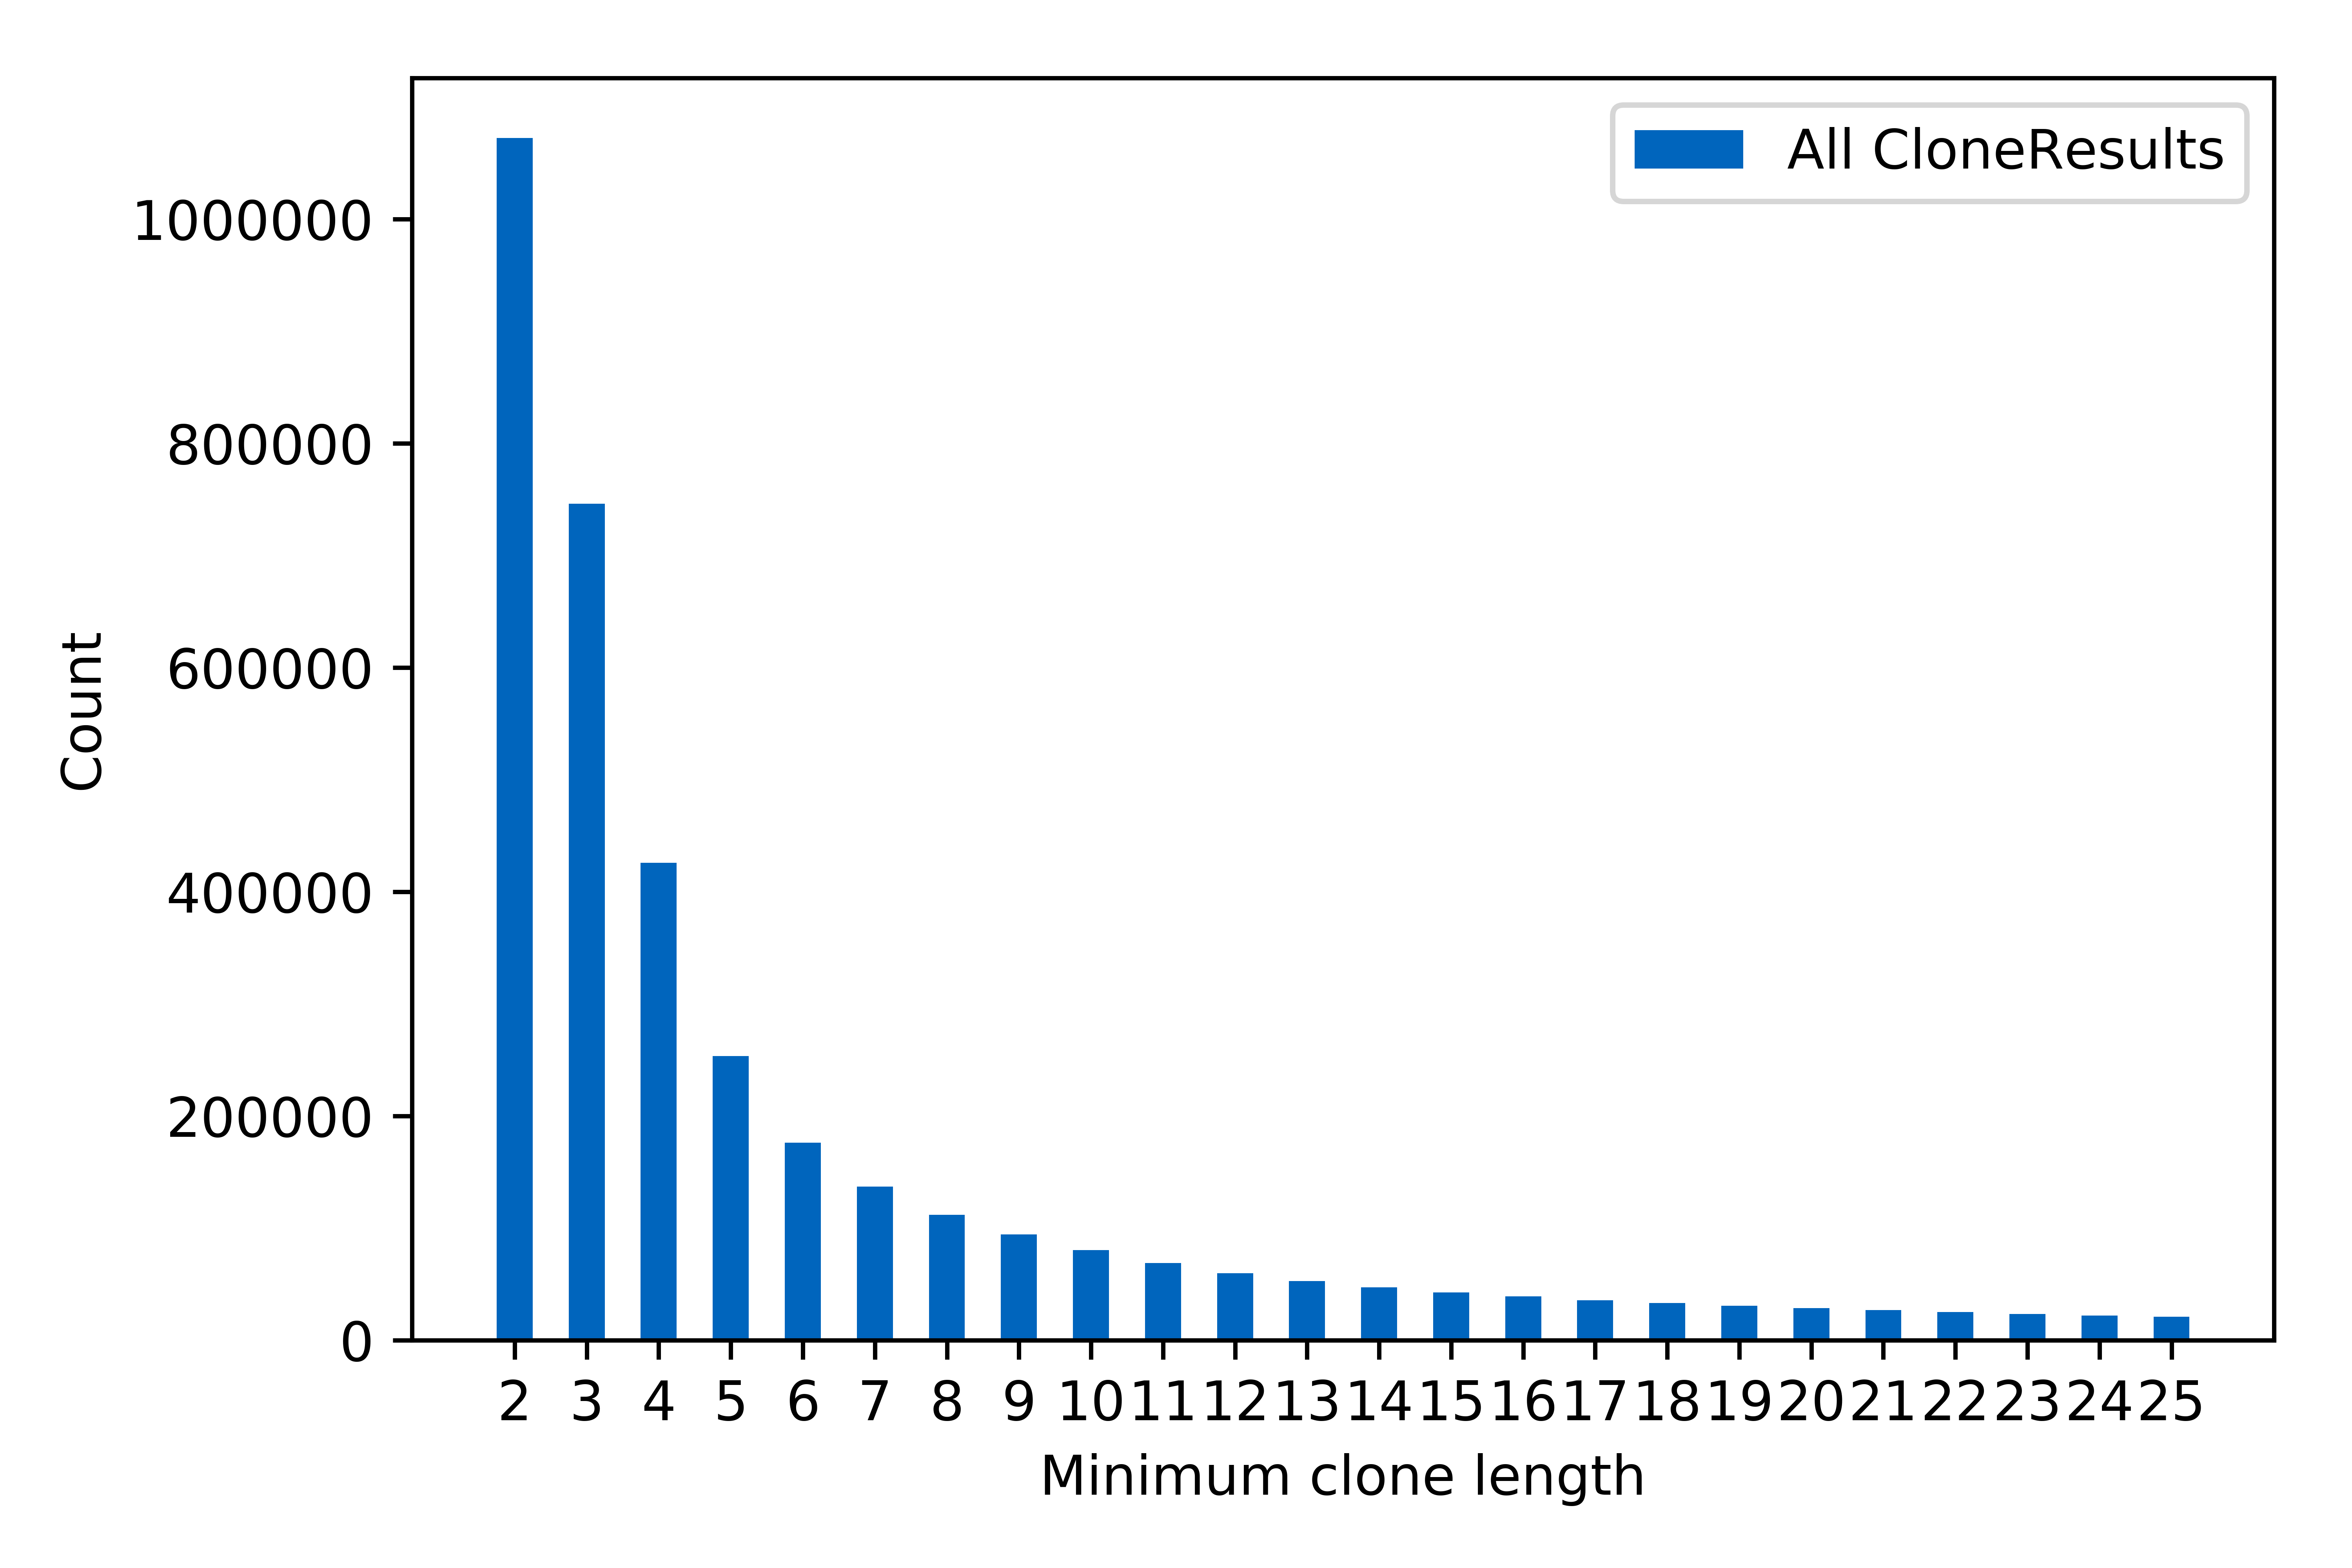
\includegraphics[width=0.8\linewidth]{figures/Thresholds/raw.png}
	\caption[All found Cloneclasses in relation to the minimum clone length]{This chart shows the number of \code{CloneResult}s found by the suffix-tree clone-detection in relation to the minimum clone length used to find them.}
	\label{fig:thresholdsAll}
\end{figure}

% !TeX root = ../../main.tex
% Add the above to each chapter to make compiling the PDF easier in some editors.

\begin{figure}
	\centering
	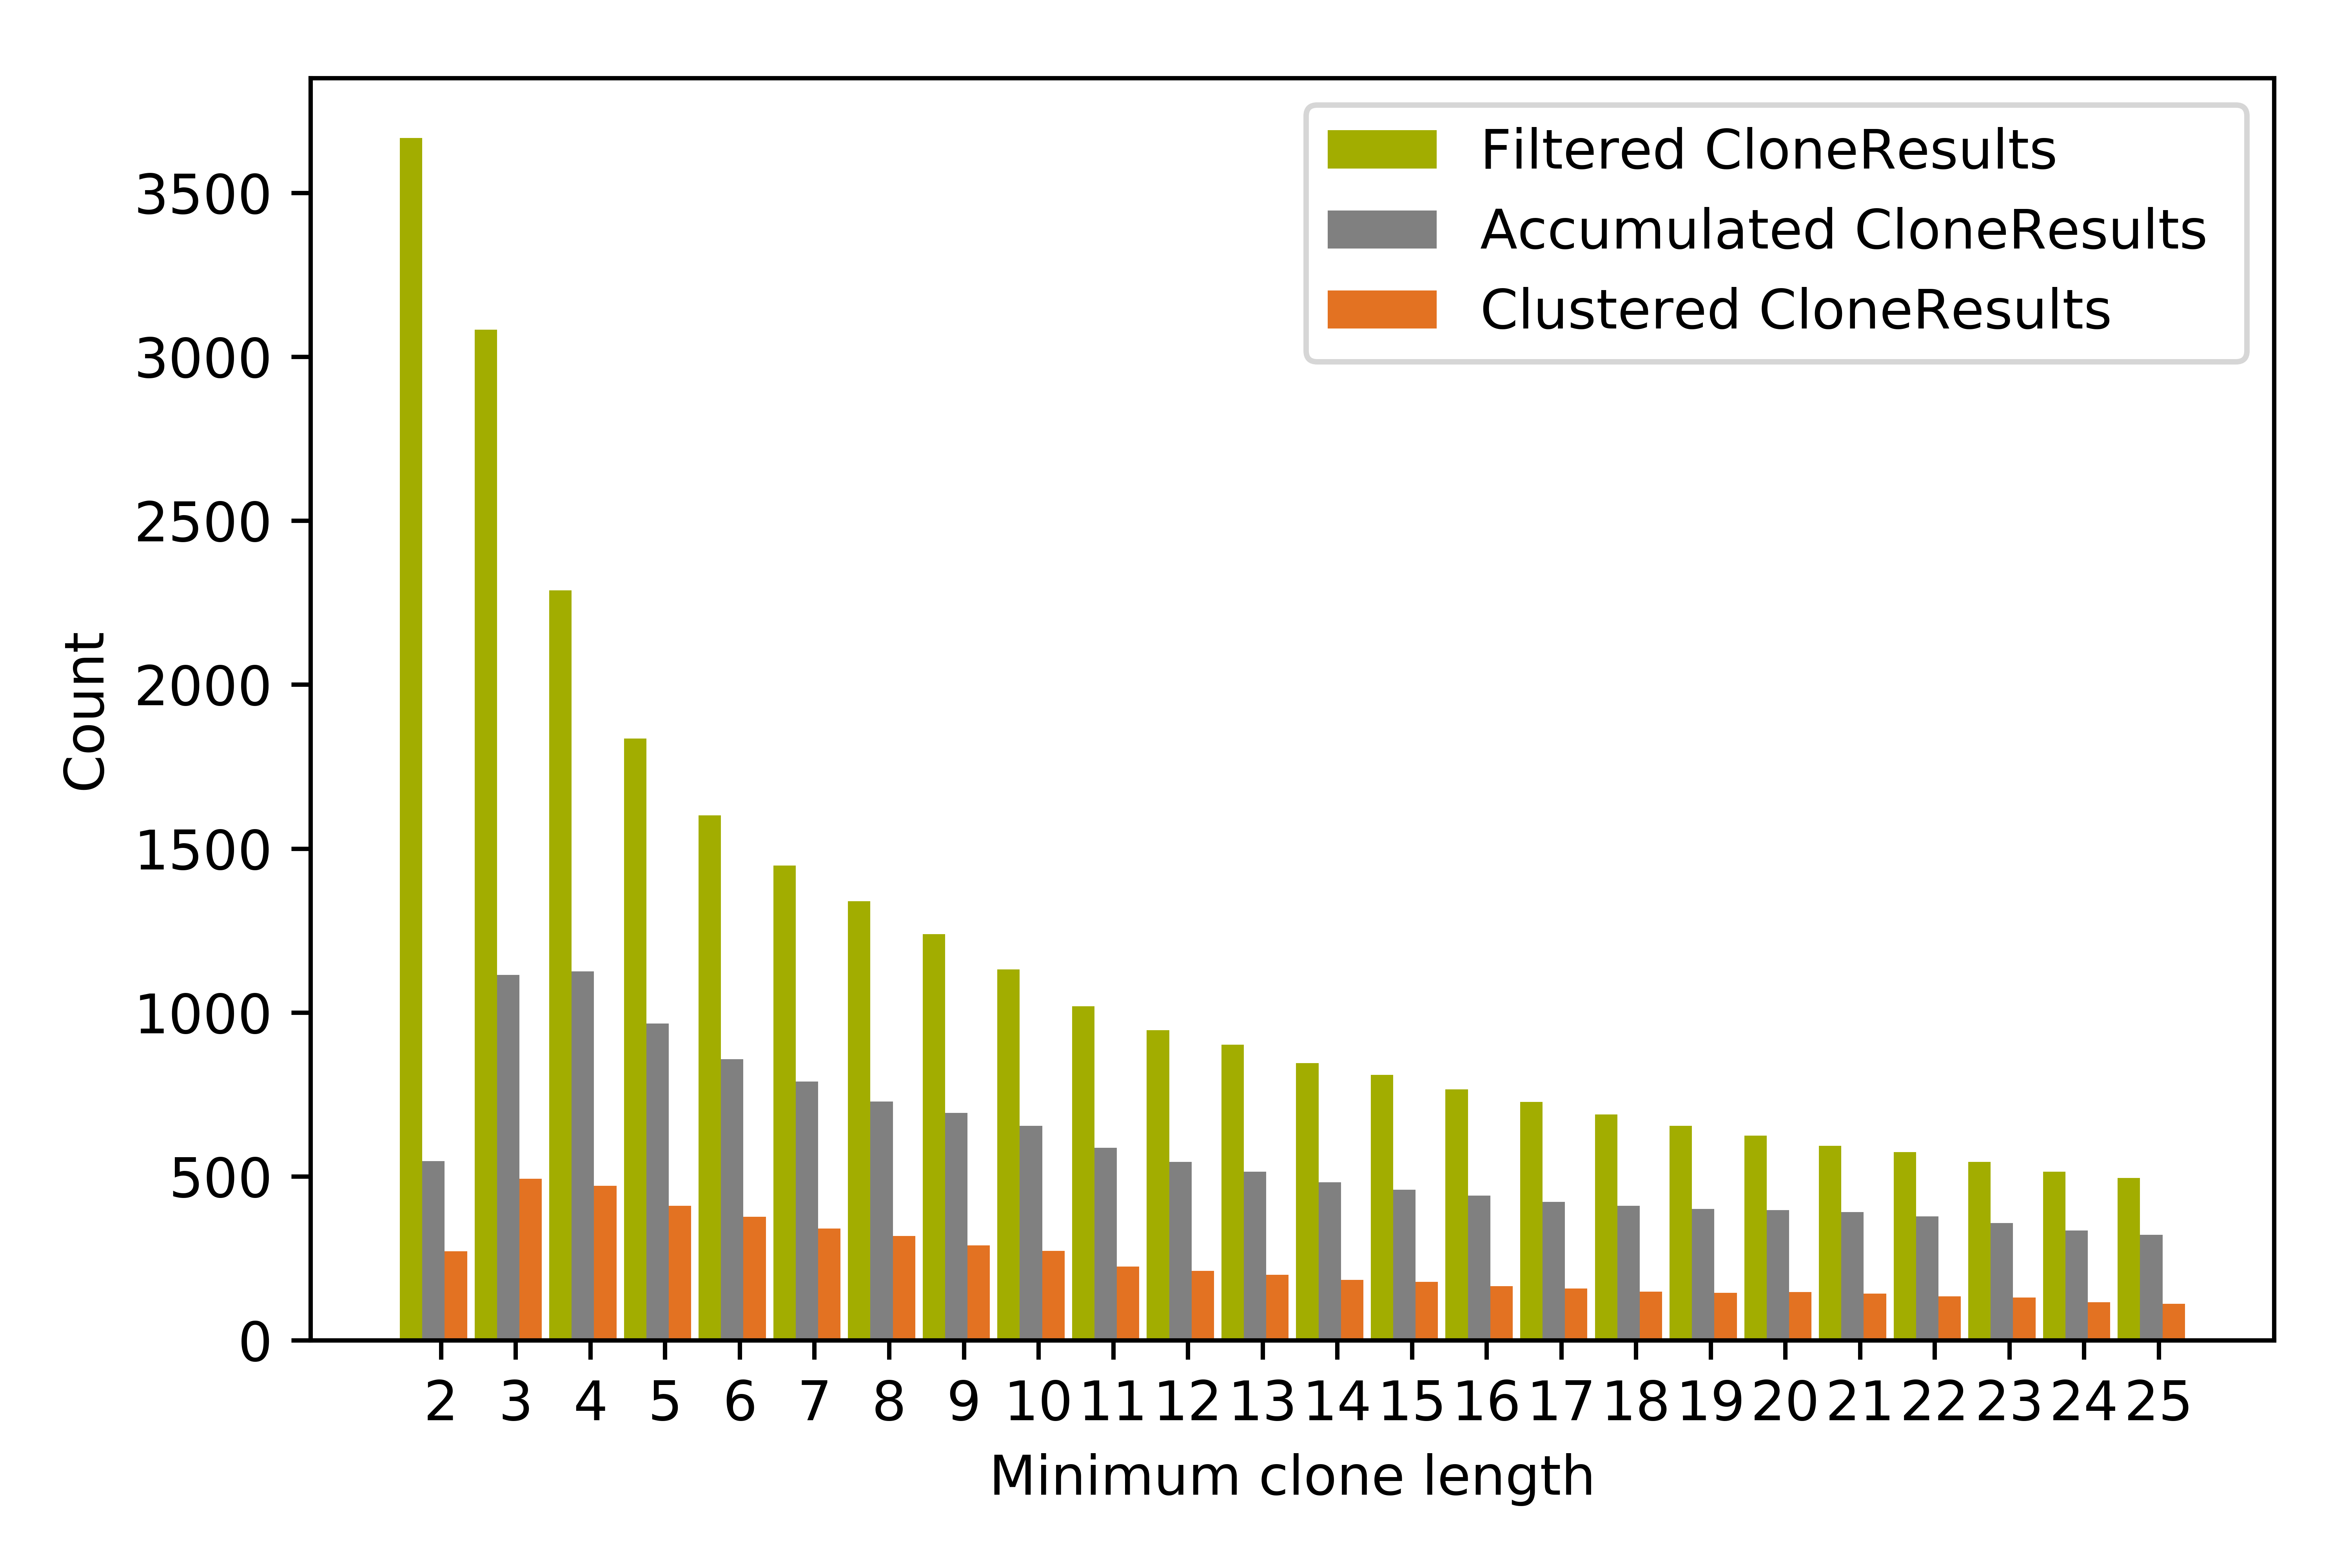
\includegraphics[width=0.8\linewidth]{figures/Thresholds/processed.png}
	\caption[Processed CloneClasses in relation to the minimum clone length]{This chart shows the number of \code{CloneResult}s that are left after the three processing steps described in Step~\ref{section:processCloneResults}. The counts are associated to their respective minimum clone length used to find the \code{CloneResult}s.}
	\label{fig:thresholdsProcessed}
\end{figure}


\subsection{Benchmarking}
\label{section:benchmark}
As displayed in Figure~\ref{fig:benchmark}, the time-intensive steps are multithreaded.\\
We performed the benchmark with a minimum clone length of 5.\\
This results in time savings ranging from 5.32\% \textit{(Get Uniform Paths)} up to 86.25\% \textit{(Create Links For: GENERATED)}. The overall time saving sums up to a total of 56.5\%, which reduces the average absolute amount of time of around 300 seconds down to 130 seconds. 
% !TeX root = ../../main.tex
% Add the above to each chapter to make compiling the PDF easier in some editors.
\begin{figure}
	\centering
	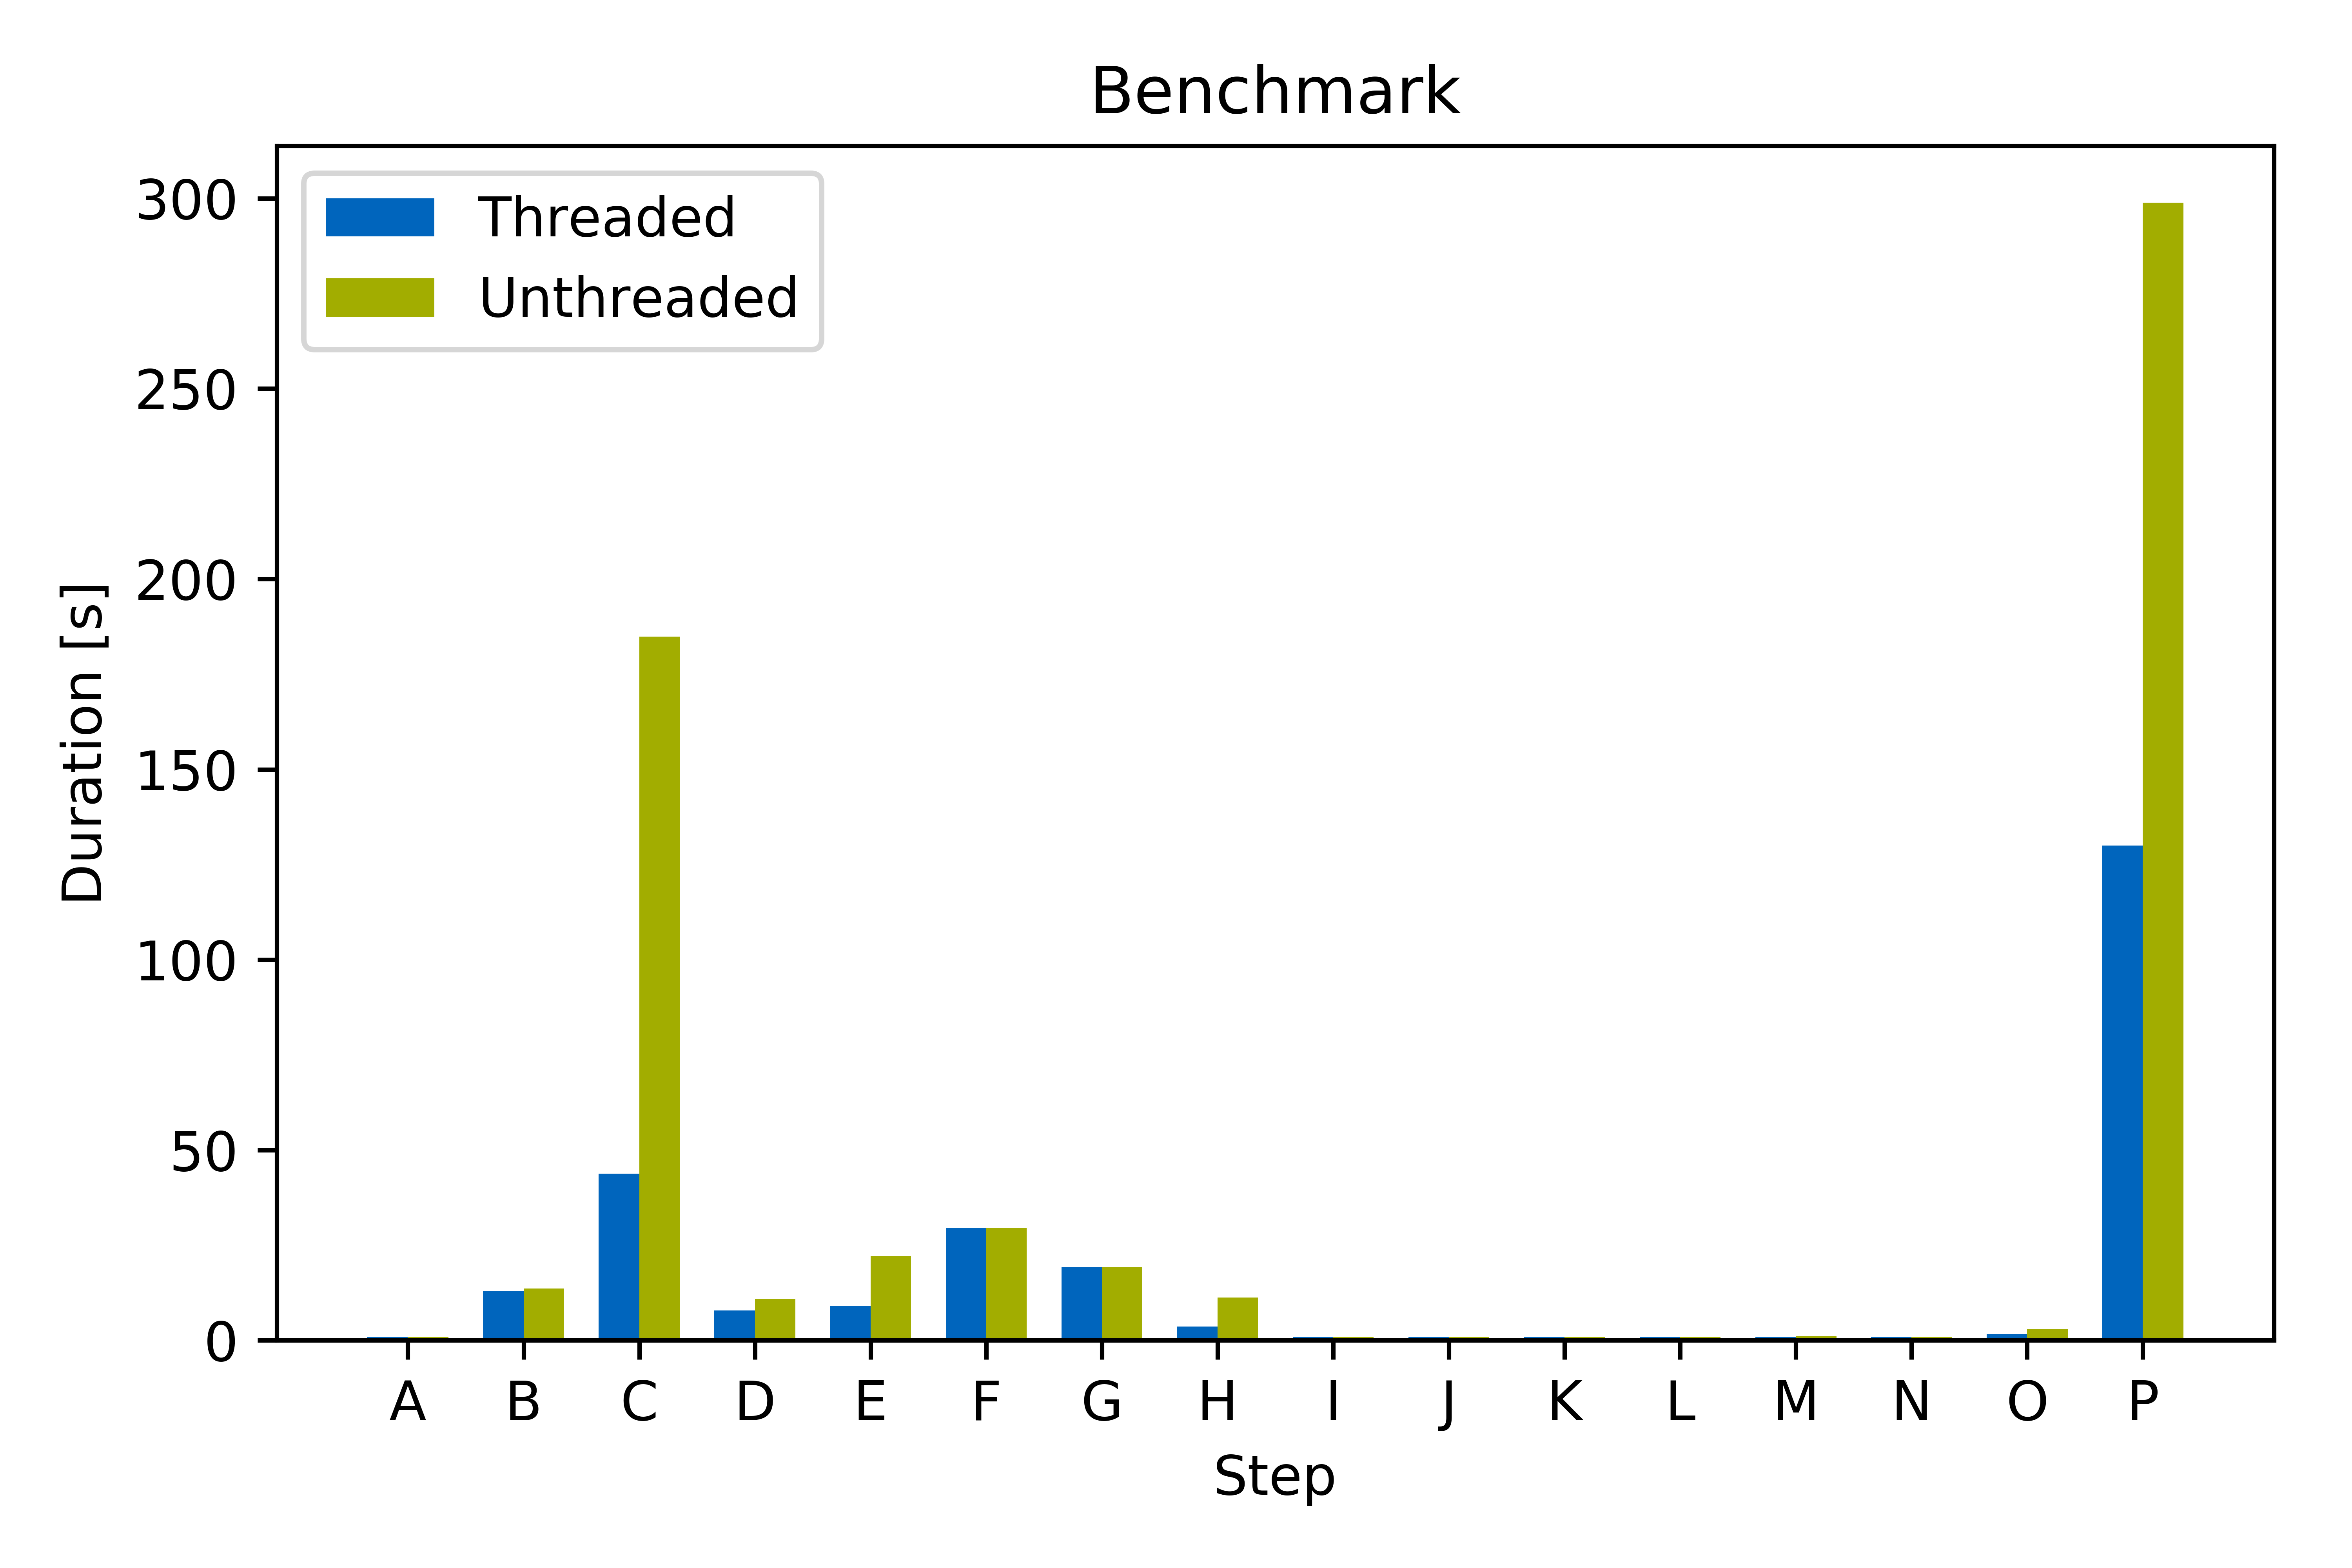
\includegraphics[width=0.8\linewidth]{figures/Benchmark/benchmark.png}
	\caption[Benchmark]{The results of the benchmarks performed during the search for generator-patterns. The step labels are explained in Table~\ref{table:tickLabels}.}
	\label{fig:benchmark}
\end{figure}
% !TeX root = ../main.tex
% Add the above to each chapter to make compiling the PDF easier in some editors.
\setlength{\extrarowheight}{.0em}
\begin{table}
	\caption{Explanation for the step labels of Figure~\ref{fig:benchmark}. The \textit{Savings} column displays the time saving gained through multithreading.}
	\label{table:tickLabels}
		\begin{tabularx}{\textwidth}{c|C|c||c|C|c}
			\textbf{Tick} & \textbf{Step} & \textbf{Savings} & \textbf{Tick} & \textbf{Step} & \textbf{Savings}\\
			\hline
			A & Get Projects & - & B & Get Uniform Paths & 5.32\% \\
			C & Retrieve Comments & 76.29\% & D & Save Comments & 27.78\% \\
			E & Prepare Comments & 59.29\% &F& Build Suffix Tree & - \\
			G& Find Clones & - & H & Convert to \code{CloneResult}s & 67.54\%\\
			I&Filter Presumable Generator Patterns & - &J&Accumulate Presumable Generator Patterns & -\\
			K&Cluster Presumable Generator Patterns & - &L&Filter Presumable Not Generator Patterns & -\\
			M& Save Files For: GENERATED& 83.06\% &N&Create Links For: GENERATED & 86.25\%\\
			O& Create Links For: NOT\_GENERATED& 42.41\% & P & Total & 56.5\%
		\end{tabularx}
\end{table}
\setlength{\extrarowheight}{0em}

\section{Results}
This section displays the results we were able to create by using the approach to find generator-patterns and by using the the resulting generator-pattern repository on the different data sets. 
\subsection{Qualitas Corpus}
At first we considered the Qualitas Corpus because it provided a good database and the results can be compared to the ones made in \cite{Bernwieser2014}.

% !TeX root = ../main.tex
% Add the above to each chapter to make compiling the PDF easier in some editors.
\setlength{\extrarowheight}{-.17em}
\begin{table}
	\caption[Lines of code distributions in the Qualitas Corpus.]{The absolute and relative proportions of lines of code in the code categories generated and manually maintained in the Qualitas Corpus.}
	\label{table:locQualitasCorpus}
	\begin{tabularx}{\textwidth}{c|r|r|r|r|r}
		& \multicolumn{5}{c}{Lines of Code}  \\
		Project & All & \multicolumn{2}{c|}{Generated} & \multicolumn{2}{c}{Manually}  \\
		\hline
		argouml & 389.952 & 11.992 & 3,08\% & 377.960 & 96,92\% \\
		axion & 41.862 & 5.417 & 12,94\% & 36.445 & 87,06\% \\
		castor & 349.301 & 18.056 & 5,17\% & 331.245 & 94,83\% \\
		cayenne & 341.902 & 15.528 & 4,54\% & 326.374 & 95,46\% \\
		cobertura & 68.154 & 51.139 & 75,03\% & 17.015 & 24,97\% \\
		compiere & 727.702 & 206.999 & 28,45\% & 520.703 & 71,55\% \\
		derby & 1.138.858 & 46.974 & 4,12\% & 1.091.884 & 95,88\% \\
		eclipse\_SDK & 4.956.920 & 103.292 & 2,08\% & 4.853.628 & 97,92\% \\
		exoportal & 146.947 & 3.353 & 2,28\% & 143.594 & 97,72\% \\
		findbugs & 185.806 & 5.895 & 3,17\% & 179.911 & 96,83\% \\
		galleon & 135.442 & 4.888 & 3,61\% & 130.554 & 96,39\% \\
		gt2 & 1.514.789 & 325.259 & 21,47\% & 1.189.530 & 78,53\% \\
		hadoop & 444.593 & 9.475 & 2,13\% & 435.118 & 97,87\% \\
		hibernate & 711.370 & 327 & 0,05\% & 711.043 & 99,95\% \\
		hsqldb & 269.978 & 1.100 & 0,41\% & 268.878 & 99,59\% \\
		ireport & 338.819 & 100.276 & 29,60\% & 238.543 & 70,40\% \\
		jag & 28.957 & 10.326 & 35,66\% & 18.631 & 64,34\% \\
		jasperreports & 347.502 & 4.978 & 1,43\% & 342.524 & 98,57\% \\
		javacc & 35.145 & 8.509 & 24,21\% & 26.636 & 75,79\% \\
		jboss & 968.808 & 8.173 & 0,84\% & 960.635 & 99,16\% \\
		jchempaint & 372.743 & 386 & 0,10\% & 372.357 & 99,90\% \\
		jedit & 176.672 & 9.575 & 5,42\% & 167.097 & 94,58\% \\
		jena & 164.679 & 5.045 & 3,06\% & 159.634 & 96,94\% \\
		jhotdraw & 133.830 & 17.062 & 12,75\% & 116.768 & 87,25\% \\
		jparse & 32.270 & 20.738 & 64,26\% & 11.532 & 35,74\% \\
		jrefactory & 301.940 & 46.449 & 15,38\% & 255.491 & 84,62\% \\
		jruby & 244.774 & 4.033 & 1,65\% & 240.741 & 98,35\% \\
		jstock & 74.361 & 30.446 & 40,94\% & 43.915 & 59,06\% \\
		lucene & 611.422 & 60.330 & 9,87\% & 551.092 & 90,13\% \\
		mvnforum & 172.855 & 32.103 & 18,57\% & 140.752 & 81,43\% \\
		myfaces\_core & 189.954 & 19.678 & 10,36\% & 170.276 & 89,64\% \\
		netbeans & 7.142.778 & 688.961 & 9,65\% & 6.453.817 & 90,35\% \\
		pmd & 80.971 & 27.671 & 34,17\% & 53.300 & 65,83\% \\
		poi & 363.487 & 21.621 & 5,95\% & 341.866 & 94,05\% \\
		sablecc & 35.388 & 21.134 & 59,72\% & 14.254 & 40,28\% \\
		struts & 261.537 & 6.978 & 2,67\% & 254.559 & 97,33\% \\
		tomcat & 352.572 & 7.356 & 2,09\% & 345.216 & 97,91\% \\
		velocity & 70.804 & 9.092 & 12,84\% & 61.712 & 87,16\% \\
		wct & 99.622 & 150 & 0,15\% & 99.472 & 99,85\% \\
		weka & 496.737 & 5.132 & 1,03\% & 491.605 & 98,97\% \\
		xalan & 354.578 & 3.217 & 0,91\% & 351.361 & 99,09\% \\
	\end{tabularx}
\end{table}
\setlength{\extrarowheight}{0em}
% !TeX root = ../main.tex
% Add the above to each chapter to make compiling the PDF easier in some editors.
\setlength{\extrarowheight}{-.15em}
\begin{table}
	\caption{The results our algorithm has created.}
	\label{table:countQualitasCorpus}
	\begin{tabularx}{\textwidth}{c|c|c|c|c|c}
		 & \multicolumn{5}{c}{Source code files}  \\
		Project & All & \multicolumn{2}{c|}{Generated} & \multicolumn{2}{c}{Manually}\\
		\hline
		argouml & 1.922 & 3 & 0,16\% & 1.919 & 99,84\% \\
		axion & 237 & 7 & 2,95\% & 230 & 97,05\% \\
		castor & 2.229 & 61 & 2,74\% & 2.168 & 97,26\% \\
		cayenne & 2.796 & 227 & 8,12\% & 2.569 & 91,88\% \\
		cobertura & 140 & 34 & 24,29\% & 106 & 75,71\% \\
		compiere & 2.508 & 681 & 27,15\% & 1.827 & 72,85\% \\
		derby & 2.842 & 17 & 0,60\% & 2.825 & 99,40\% \\
		eclipse\_SDK & 22.263 & 235 & 1,06\% & 22.028 & 98,94\% \\
		exoportal & 1.839 & 23 & 1,25\% & 1.816 & 98,75\% \\
		findbugs & 1.062 & 7 & 0,66\% & 1.055 & 99,34\% \\
		galleon & 255 & 19 & 7,45\% & 236 & 92,55\% \\
		gt2 & 7.097 & 1.493 & 21,04\% & 5.604 & 78,96\% \\
		hadoop & 1.988 & 14 & 0,70\% & 1.974 & 99,30\% \\
		hibernate & 6.214 & 1 & 0,02\% & 6.213 & 99,98\% \\
		hsqldb & 514 & 1 & 0,19\% & 513 & 99,81\% \\
		ireport & 1.626 & 235 & 14,45\% & 1.391 & 85,55\% \\
		jag & 132 & 20 & 15,15\% & 112 & 84,85\% \\
		jasperreports & 1.589 & 10 & 0,63\% & 1.579 & 99,37\% \\
		javacc & 195 & 40 & 20,51\% & 155 & 79,49\% \\
		jboss & 6.806 & 199 & 2,92\% & 6.607 & 97,08\% \\
		jchempaint & 2.042 & 5 & 0,24\% & 2.037 & 99,76\% \\
		jedit & 531 & 11 & 2,07\% & 520 & 97,93\% \\
		jena & 914 & 18 & 1,97\% & 896 & 98,03\% \\
		jhotdraw & 613 & 67 & 10,93\% & 546 & 89,07\% \\
		jparse & 75 & 7 & 9,33\% & 68 & 90,67\% \\
		jrefactory & 2.229 & 140 & 6,28\% & 2.089 & 93,72\% \\
		jruby & 1.128 & 9 & 0,80\% & 1.119 & 99,20\% \\
		jstock & 274 & 52 & 18,98\% & 222 & 81,02\% \\
		lucene & 3.036 & 89 & 2,93\% & 2.947 & 97,07\% \\
		mvnforum & 705 & 100 & 14,18\% & 605 & 85,82\% \\
		myfaces\_core & 1.052 & 60 & 5,70\% & 992 & 94,30\% \\
		netbeans & 32.567 & 1.864 & 5,72\% & 30.703 & 94,28\% \\
		pmd & 751 & 162 & 21,57\% & 589 & 78,43\% \\
		poi & 2.007 & 14 & 0,70\% & 1.993 & 99,30\% \\
		sablecc & 198 & 135 & 68,18\% & 63 & 31,82\% \\
		struts & 1.836 & 43 & 2,34\% & 1.793 & 97,66\% \\
		tomcat & 1.324 & 44 & 3,32\% & 1.280 & 96,68\% \\
		velocity & 371 & 9 & 2,43\% & 362 & 97,57\% \\
		wct & 638 & 1 & 0,16\% & 637 & 99,84\% \\
		weka & 1.271 & 9 & 0,71\% & 1.262 & 99,29\% \\
		xalan & 975 & 2 & 0,21\% & 973 & 99,79\% \\
	\end{tabularx}
\end{table}
\setlength{\extrarowheight}{0em}

\subsubsection{Lines of code for generated and manually maintained source code.}
- 
\subsubsection{Number of generated and manually maintained source code files.}
- 
\subsubsection{Ratio of generated to manually maintained source code and files.}
- 
\subsubsection{Amount of generated code detected by our approach compared to the one used in \cite{Bernwieser2014}.}
- 
\subsection{Random Git Projects}
a
\section{Discussion}
a
\subsection{Completeness and accuracy}
a
\subsection{Relevance of results}
a
\section{Threats to validity}
a
\subsection{Wrong filtering}
a
\subsection{Minimum clone length vs. irrelevant data}
a
\subsection{Representativeness of data sets}
a
\subsection{Generators without pattern}
a